\documentclass{cccg10}
\usepackage{graphicx,amssymb,amsmath}

\usepackage{subfigure}
%----------------------- Macros and Definitions --------------------------

% Add all additional macros here, do NOT include any additional files.

% The environments theorem (Theorem), invar (Invariant), lemma (Lemma),
% cor (Corollary), obs (Observation), conj (Conjecture), and prop 
% (Proposition) are already defined in the cccg10.cls file.
% Add additional environments only if you REALLY need them.

%----------------------- Title -------------------------------------------

\DeclareMathOperator{\od}{d}
\DeclareMathOperator{\vol}{v}
\DeclareMathOperator{\cog}{c}
\newcommand{\drop}{\downarrow}
\newcommand{\R}{\mathbb{R}}

\newcommand{\eqlabel}[1]{\label{eq:#1}}
\renewcommand{\eqref}[1]{(\ref{eq:#1})}



\title{Oja Medians and Centers of Gravity}

\author{Dan Chen\thanks{School of Computer Science,
        Carleton University, \texttt{morin@scs.carleton.ca}}
        \and
        Olivier Devillers
        \and
        John Iacono
        \and
        Stefan Langerman
        \and
        Pat Morin\footnotemark[1]}
        
% Add the appropriate index information!        
        
\index{Chen, Dan}
\index{Morin, Pat}

%------------------------------ Text -------------------------------------

\begin{document}
\thispagestyle{empty}
\maketitle


\begin{abstract}
The relationships between the Oja median and centers of gravity are
considered.
\end{abstract}

\section{Introduction}

Given a set $S$ of $n$ points in $\mathbb{R}^{d}$, the \emph{Oja depth}
\cite{Oja83} of a point $x\in\R^d$ is
\[ 
   \od(x, S) 
      = \sum_{y_{1},\ldots , y_{d} \in \binom{S}{d}} 
         \vol(x, y_{1}, \ldots, y_{d}) \enspace ,
\]
where $\vol(p_{1},\ldots, p_{d+1})$ denotes the volume of the simplex
whose vertices are $p_{1}\ldots p_{d+1}$.\footnote{In Oja's original
definition, the sum is normalized by dividing by $\binom{|S|}{d}$. We omit this here since it changes none of our results and clutters our formulas.}
A point in $\mathbb{R}^{d}$ with the minimum Oja depth is called an
\emph{Oja center}.

\subsection{New Results}

In this paper we consider relationships between centers of gravity of
certain sets and Oja depth. The \emph{center of gravity} of a finite
point set $S\subset\R^d$ is the average of those points,
\[
  \cog(S) = |S|^{-1}\sum_{x\in S} x \enspace .
\]
If $P\subset\R^d$ is a bounded object of non-zero volume, the center of gravity of $P$ is
\[
  \cog(P) = \frac{\int_{\R^d} x P(x) dx}{\int_{\R^d} P(x) dx}
\]
where $P(\cdot)$ is the characteristic function of $P$, so $P(x)=1$ if $x\in P$ and $P(x)=0$ otherwise.

In this paper, we prove the following results about the Oja depth of an
$n$ point set $S$, whose convex hull $A$ has unit volume and that has an Oja center $x$:

\begin{equation}
  \od(\cog(A),S) \le \binom{n}{d}/(d+1) \enspace ,
   \eqlabel{centerpoint}
\end{equation}
\begin{equation}
  \od(\cog(S),S) \le (d+1)\od(x,S) \enspace .
   \eqlabel{approx}
\end{equation}

\subsection{Related Results}

Our first result, \eqref{centerpoint}, is a form of \emph{Centerpoint
Theorem} that upper-bounds the Oja depth of $\cog(A)$, and hence
also the Oja depth $x$, in terms of the volume of the convex hull
of $S$.  Previously, centerpoint theorems were known for other depth
functions such as Tukey depth \cite{m02,pa95,t71} and simplicial depth
\cite{b82,bf84,l90}.  To the best of our knowledge, this is the first
such result for Oja depth.

Our next result, \eqref{approx}, can be viewed in two
ways.  The first is as a linear-time constant factor approximation for
finding an Oja median. 

In 1-d, Oja depth is minimized by the median, which can be found in $O(n)$
time. However, in 2-d, the best known algorithm for minimizing Oja depth
exactly takes $O(n\log^3 n)$ time \cite{alst03}.  Approximation algorithms
for minimizing Oja depth, based on uniform grids and sampling from
$\binom{S}{d}$, are given by Ronkainen, Oja, and Orponen \cite{roo01}.
However, in pathological cases, their approximation algorithm is not
guaranteed (or even likely) to find a point that closely approximates
the Oja median, either in terms of distance or in terms of its Oja
depth.\footnote{This follows from the fact that the value of the Oja depth
function and the location of the Oja median can be arbitrarily different
for two sets $S_1$ and $S_2$ that differ in only $d$ points \cite{not90}.}

Another view of \eqref{approx} is that it gives insight into
the Oja depth function and the Oja median.  In some sense, they tell us
that the Oja median is not terribly different from the center of gravity
of $S$, since the center of gravity of $S$ minimizes, to within a constant factor, the Oja depth function.

\section{Oja Center and the Gravity Center of $A$}
%\label{sec:cnterofA}
\label{sec:gravcenter}

In this section, we relate the Oja depth of the center of gravity of the
convex hull of $S$ to the volume of the convex hull of $S$.  Throughout
this section, $A$ denotes the convex hull of $S$ and we assume, without
loss of generality, that $\vol(A)=1$.

Our upper-bound is based on the following identity:  For any disjoint sets
$X,Y\subseteq\R^d$, 
\[\cog(X \cup Y) = \frac{\vol(X)\cog(Y) + \vol(Y)\cog(Y)}{\vol(X \cup Y)}.\]


%\subsection{An Upper Bound in $\mathbb{R}^{2}$}
%\label{sec:2dbound}
%
%\begin{lemma}
%  \label{lem:2dgrav}
%  Let $E$ be a convex polygon, let $g_{e}$ be the gravity center of $E$, and let $y_{1}, y_{2}$ be any two points in $E$. Then $\vol(y_{1}y_{2}g_{e}) \leq \frac{1}{3} \vol(E)$.
%\end{lemma}
%\begin{proof}
%  We first show that after a sequence of transformations, we can get a
%triangle with the same area as $E$ and its gravity center is further from
%the segment $y_1y_2$ than the center of gravity of $E$. Suppose $E$ is the convex hull shown in Figure~\ref{fig:2da}, edge $af$ is parallel to the $x$-axis, and $g_{e}$ is the gravity center of $E$.
%\begin{figure}[ht]
%  \centering
%  \subfigure[]{\label{fig:2da}
%    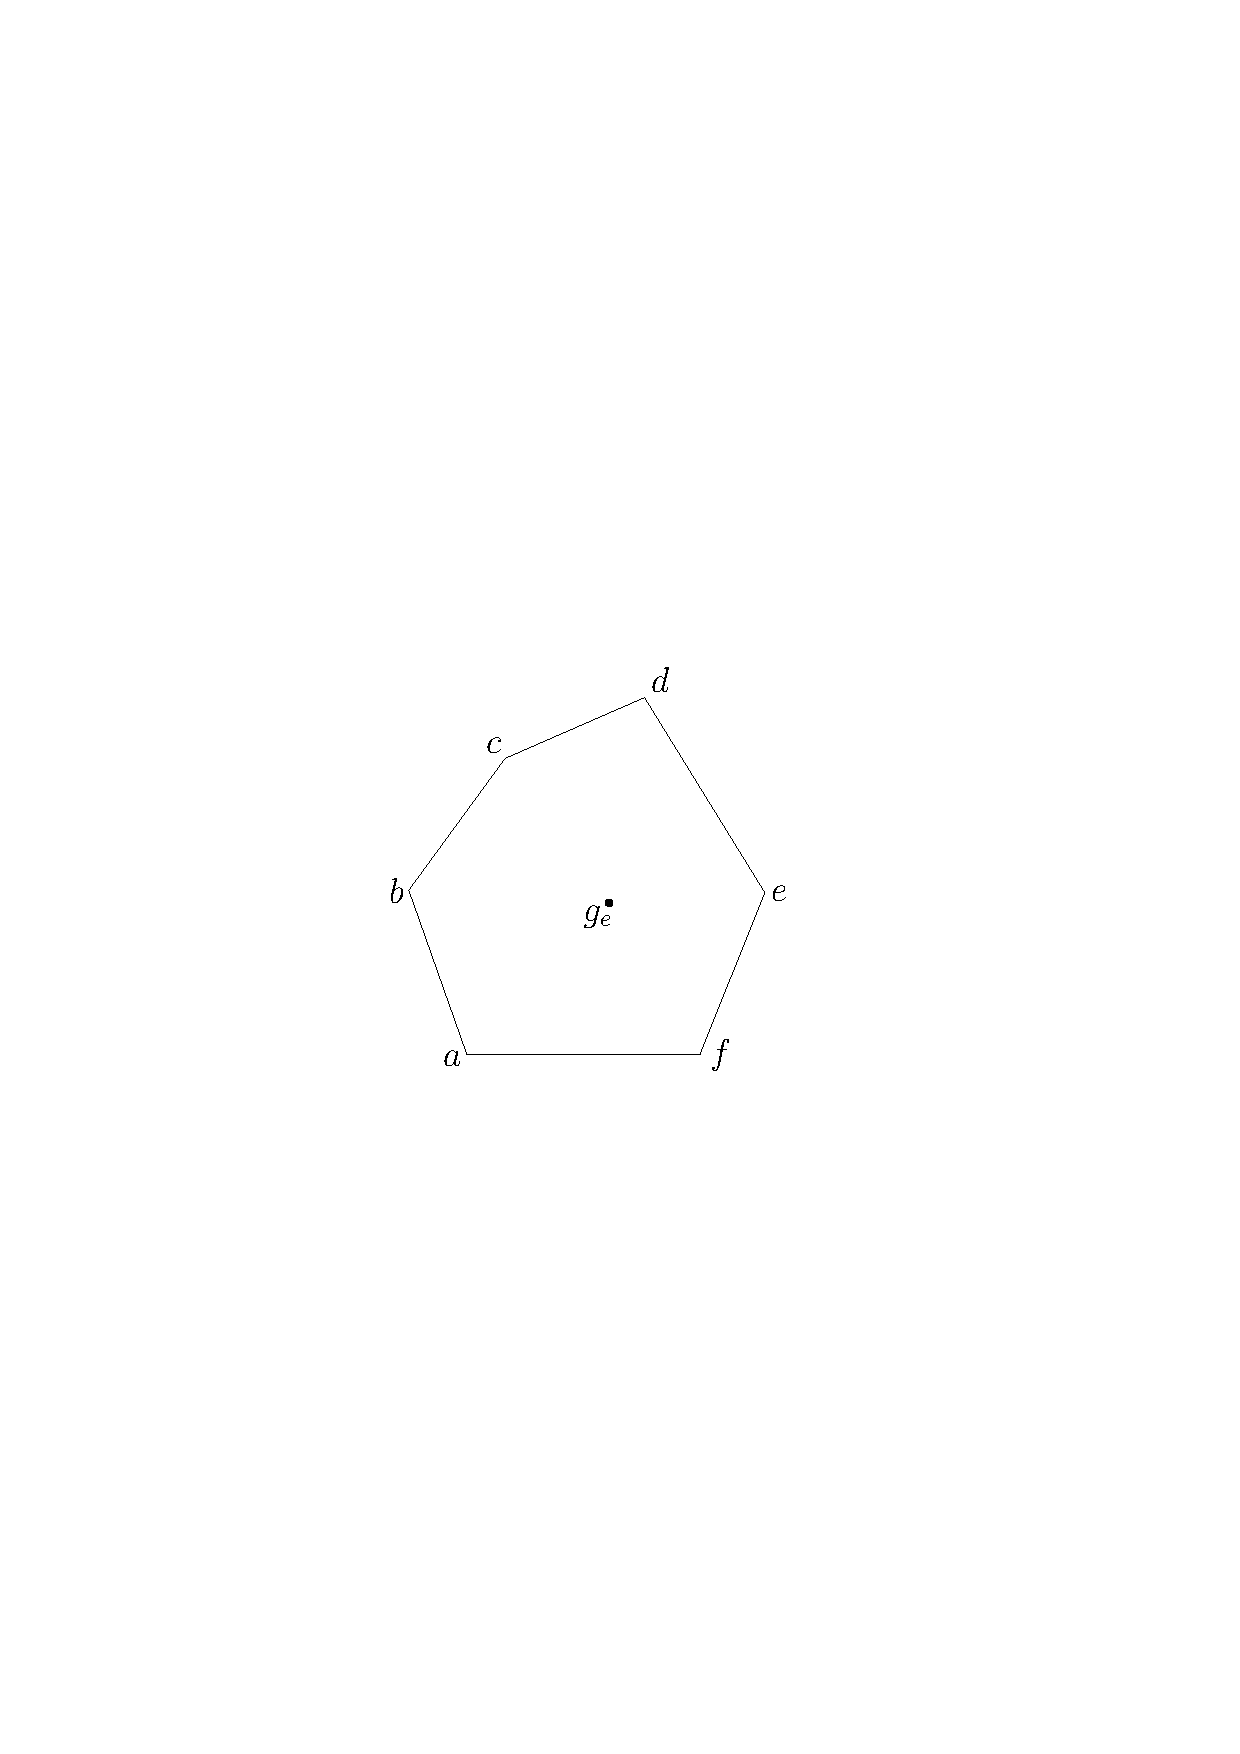
\includegraphics[width=0.20\textwidth]{pics/2da.pdf}
%  }
%  \subfigure[]{\label{fig:2db}
%    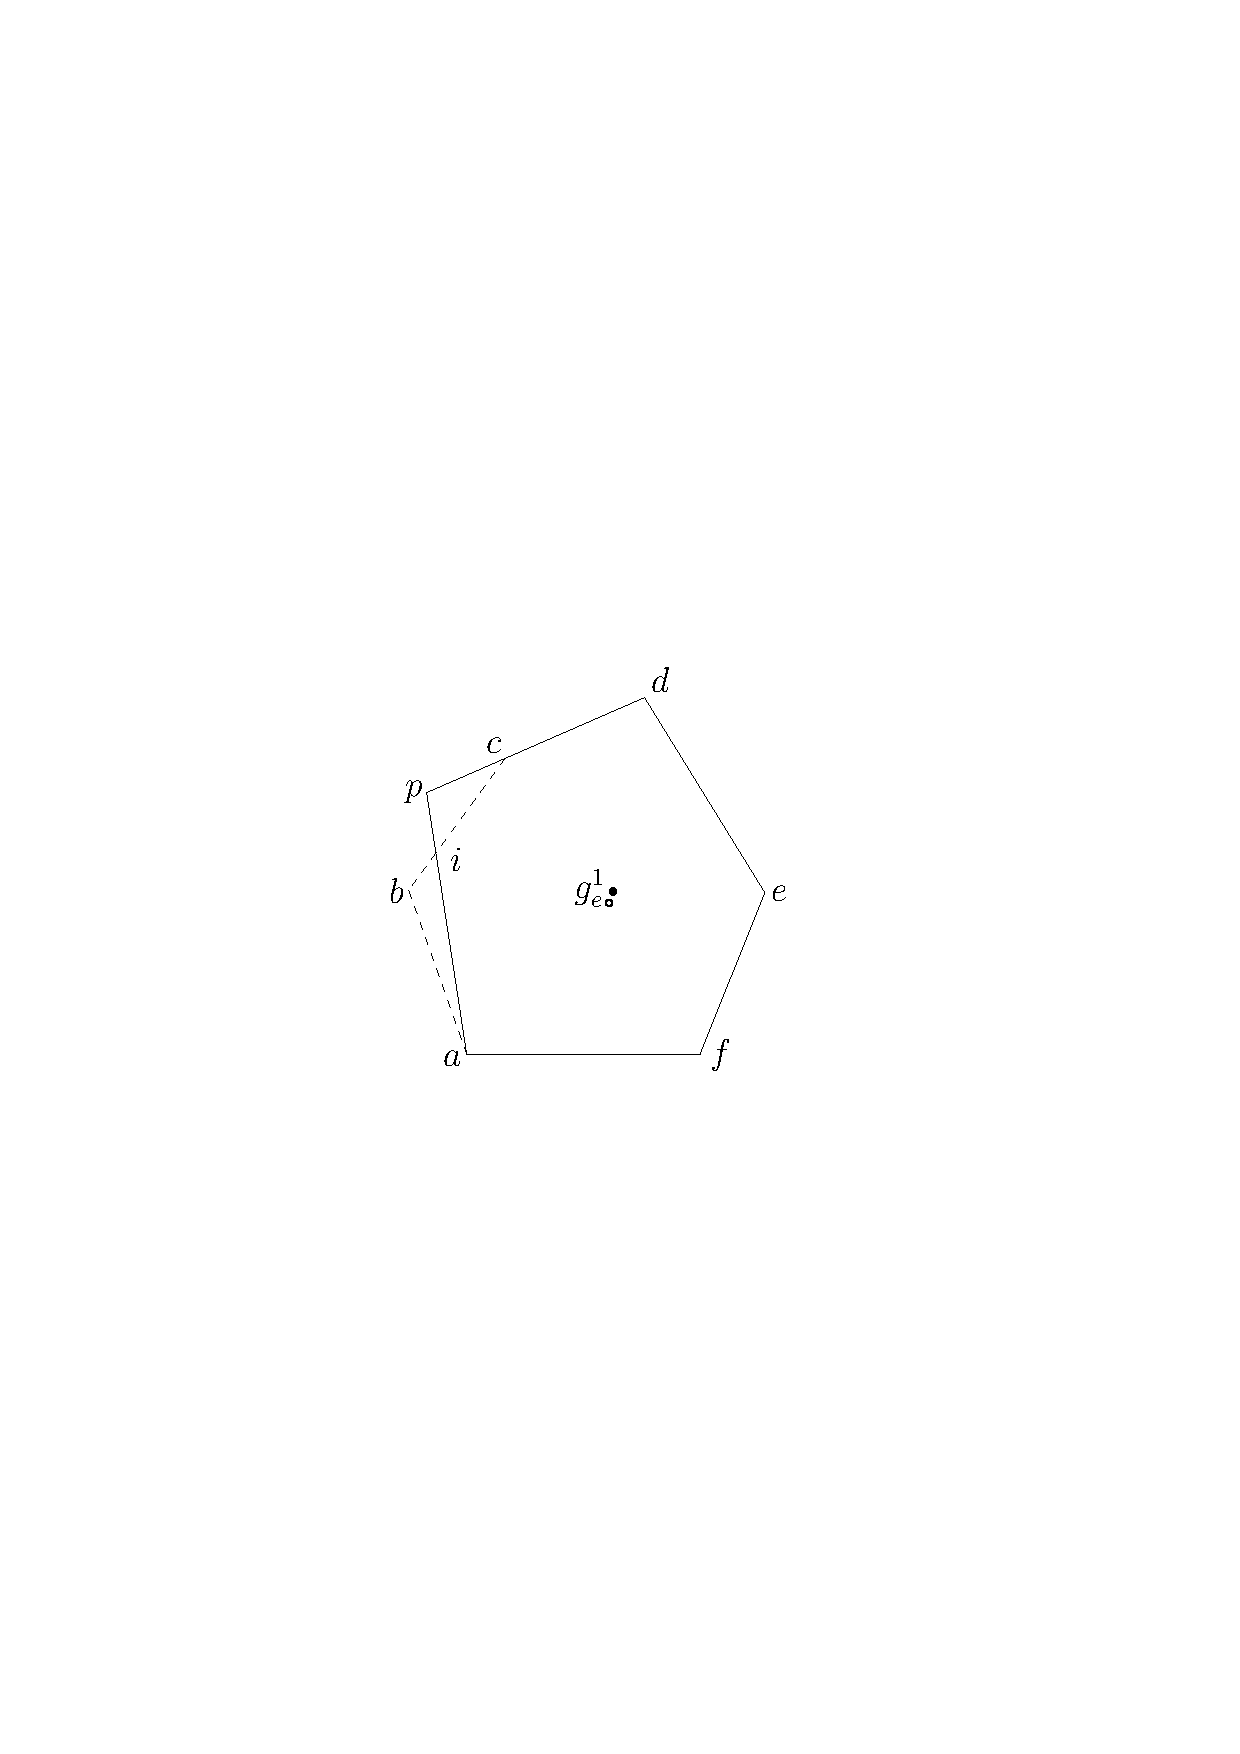
\includegraphics[width=0.20\textwidth]{pics/2db.pdf}
%  }
%  \subfigure[]{\label{fig:2dc}
%    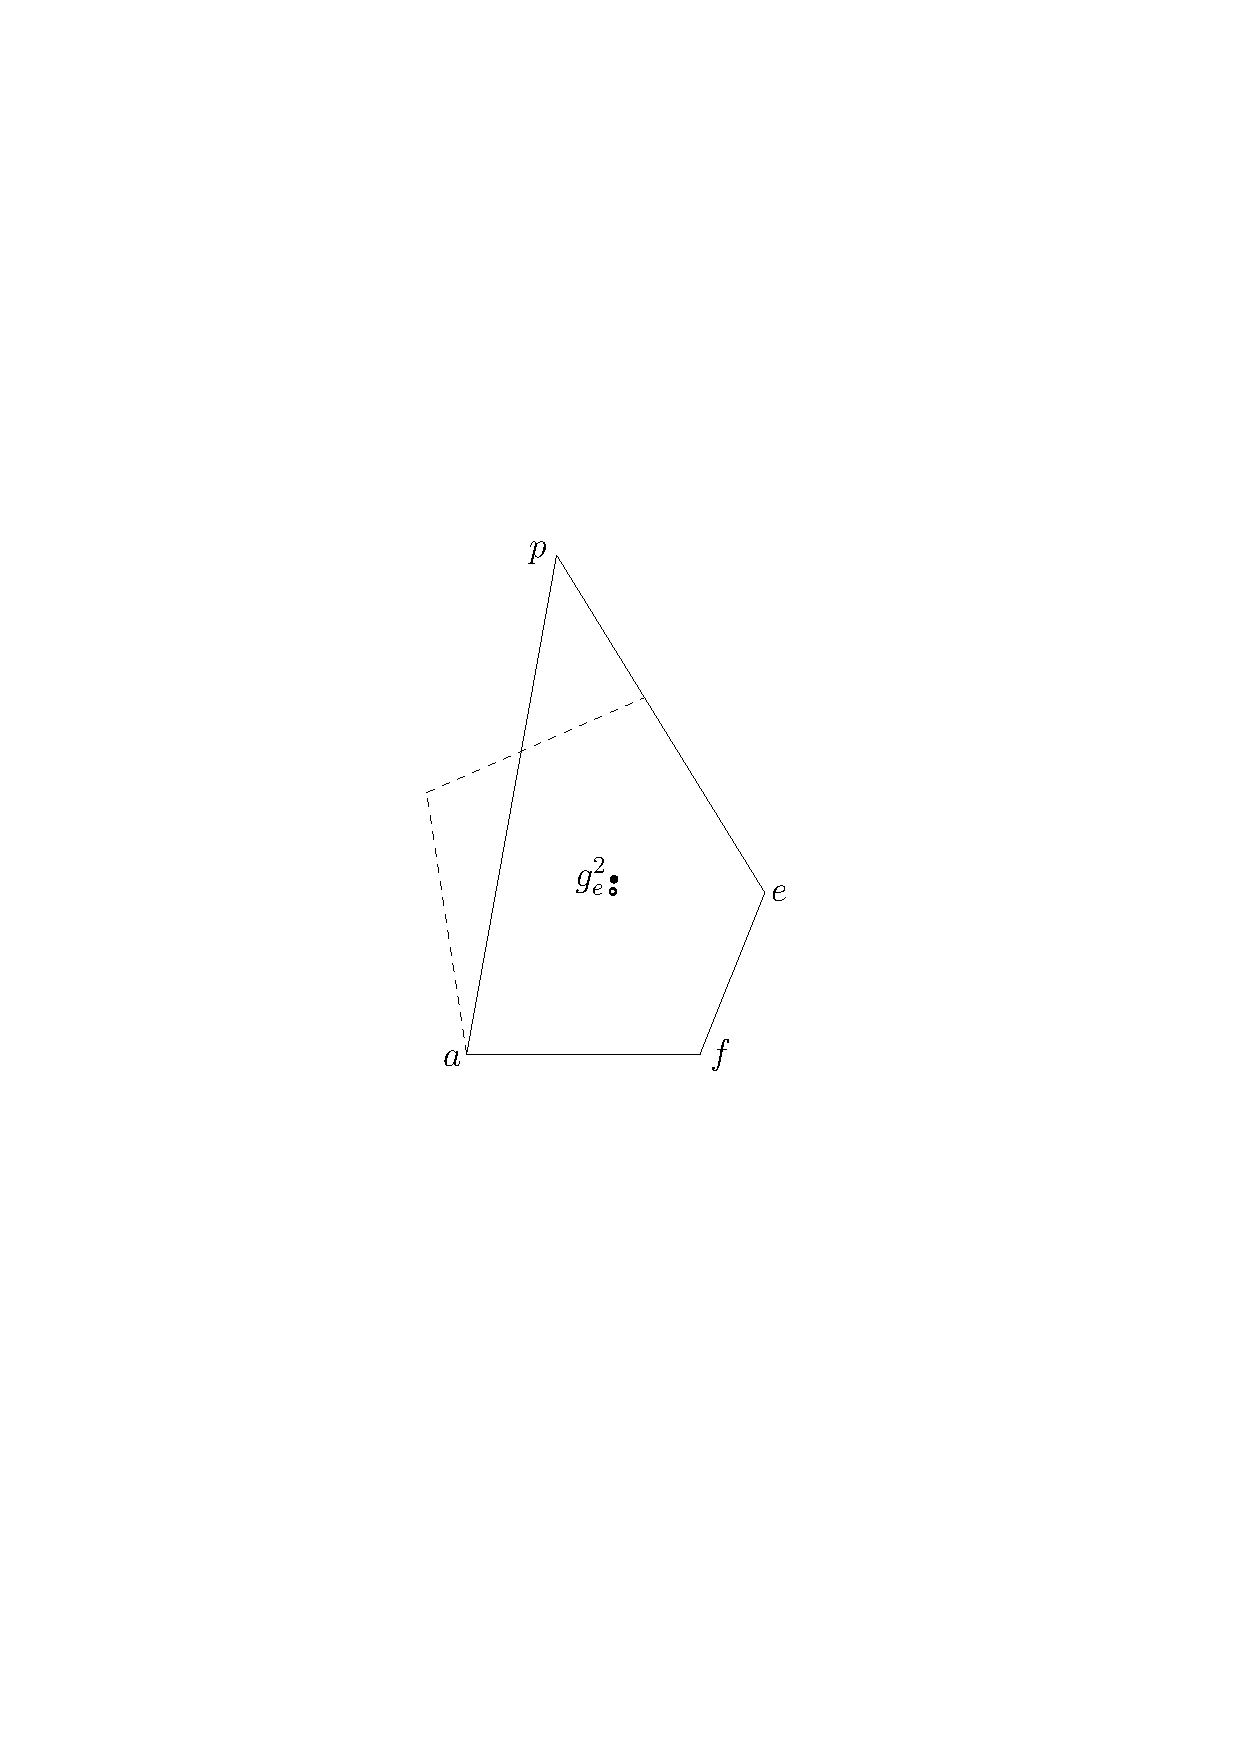
\includegraphics[width=0.18\textwidth]{pics/2dc.pdf}
%  }
%  \subfigure[]{\label{fig:2dd}
%    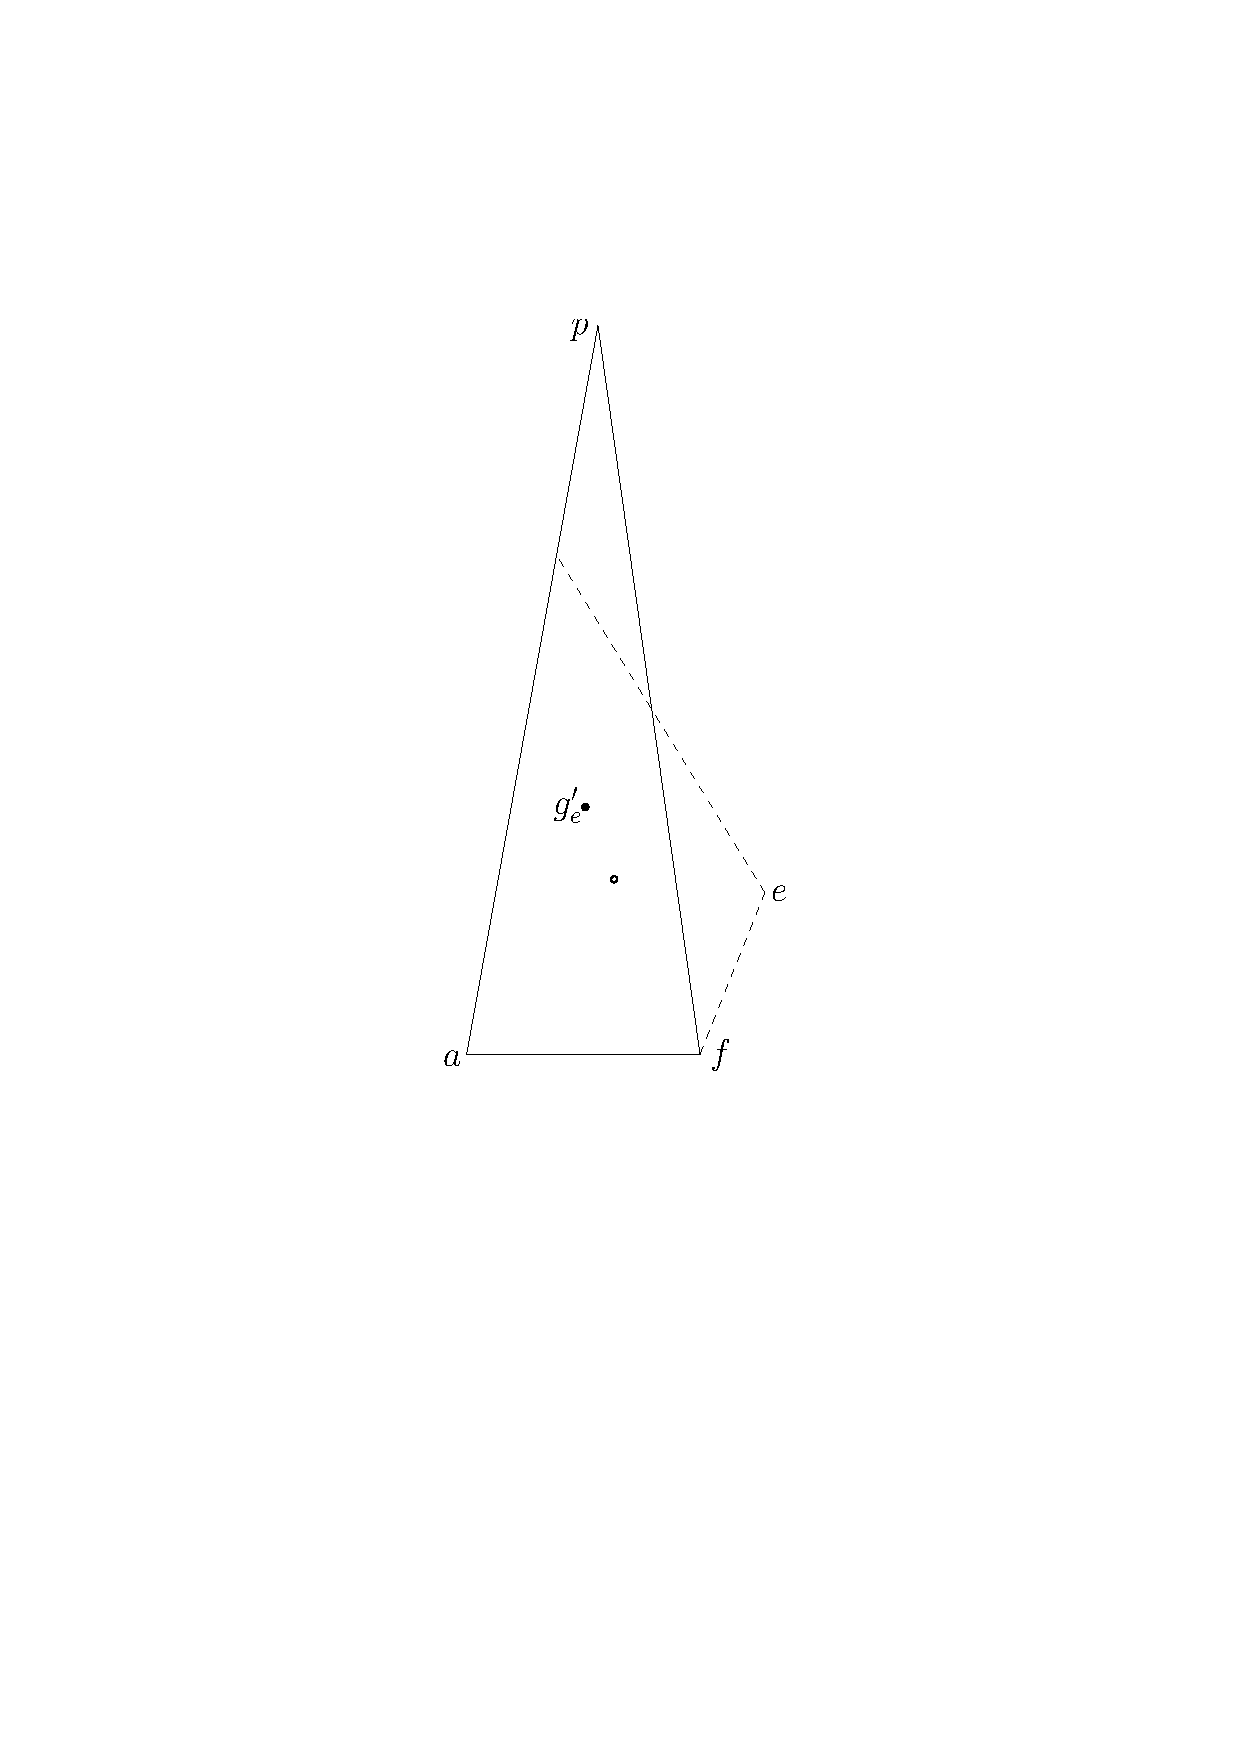
\includegraphics[width=0.17\textwidth]{pics/2dd.pdf}
%  }
%  \caption{The sequence of transformations in $\mathbb{R}^{2}$}
%  \label{fig:2dtrans}
%\end{figure}
%In the first step, as shown in Figure~\ref{fig:2db}, we extend $dc$ to point $p$ such that the area of $\triangle cpi$ equals that of $\triangle abi$, where $i$ is the intersection of $ap$ and $bc$. Now the new convex hull $apdef$ has the same area as the original $E$. Since $\triangle cpi$ is above $i$ and $\triangle abi$ is below $i$. The gravity center of the new convex hull will move up after the transformation. Continuing to do the same transformation on the same side of $E$ until $p$ becomes the highest extreme point (Figure~\ref{fig:2dc}), we start from the other side of $E$. After all transformations, we will get triangle with the same area as $E$ and whose gravity center $g_{e}'$ is above that of $E$ (Figure~\ref{fig:2dd}).
%
%Therefore, $\vol(afg_{e}) \leq \vol(afg_{e}') = \frac{1}{3} \vol(E)$. In other words, the area of any triangle formed by an edge of $E$ and $g_{e}$ no more than $\frac{1}{3} \vol(E)$.
%
%Let $y_{1}, y_{2}$ be two ponts in $E$, and $a, b$ be the intersection of $E$ and the line $l$ throuth $y_{1}$ and $y_{2}$. Line $l$ divides $E$ into two convex polygons. If $g_{e}$ is on $l$, $\vol(y_{1}y_{2}g_{e}) = 0$, otherwise, let $E'$ be the one that contains $g_{e}$ and $E''$ be other one. Let $g'$ and $g''$ be the gravity centers of $E'$ and $E''$ respectively. Since $g_{e}$ is the normalized weighted sum of $g'$ and $g''$, $g'$ can not be closer to $l$ comparing with $g_{e}$. Then
%\[\vol(y_{1}y_{2}g_{e}) \leq \vol(abg_{e}) \leq \vol(abg') \leq \frac{1}{3} \vol(A') \leq \frac{1}{3}. \]
%\end{proof}
%
%\begin{theorem}
%  \label{thm:2dcenter}
%  In $\mathbb{R}^{2}$, the gravity center of $A$ has depth value no more than $\frac{n^{2}}{6}$.
%\end{theorem}
%
%\begin{proof}
%  According to Lemma~\ref{lem:2dgrav},
%\[\od(\cog(A), S) = \sum_{y_{1}, y_{2}\in \binom{S}{2}} \vol(y_{1}y_{2}\cog(A)) \leq \frac{n^{2}}{6}.\]
%\end{proof}
%
%
%\subsection{An Upper Bound  in  $\mathbb{R}^{d}$}


First let us introduce a notion from convex geometry. Let $A$ be a convex body in $\mathbb{R}^{d}$, where $d \geq 2$. Suppose $A$ lies between parallel hyperplanes $x_{1} = a$ and $x_{1} = b$, where $a < b$. For each $x$ with $a \leq x \leq b$, let $A_{x}$ be the intersection of $A$ with the hyperplane $x_{1} = x$, and define $r_{x}$ by the equation
\[ \omega_{d-1}r_{x}^{d-1} = \vol_{d-1}(A_{x}), \]
where $\vol_{d-1}(X)$ denotes the $(d-1)$-dimensional volume of $X$ and
$\omega_{d-1}$ is the $(d-1)$-dimensional volume of the unit $(d-1)$-ball.
In this way, $r_{x}$ is the radius of a $(d-1)$-ball whose $\vol_{d-1}$-volume is the same as that of $A_{x}$. For each $a \leq x \leq b$, let $C_{x}$ be defined by the equation
\[ C_{x} = \{ (x, x_{2}, \ldots, x_{d}) : x_{2}^{2} + \cdots + x_{d}^{2} \leq r_{x}^{2} \}. \]
Then the set
\[ C = \cup (C_{x} : a \leq x \leq b) \]
is called the \emph{Schwarz rotation-symmetral} of $A$ in the $x_{1}$-axis.
For example, in $\R^3$, $C$ is a stack of disks perpendicular to, and
centered on, the $x$-axis. Each disk has the same area as the corresponding
slice of $A$.

\begin{theorem}[Webster~\cite{Webs95}]
  \label{thm:webs}
  Let $A$ be a convex body in $\mathbb{R}^{d}$ $(d \geq 2)$ whose Schwarz rotation-symmetral in the $x_{1}$-axis is $C$. Then $C$ is a convex body having the same volume as $A$.
\end{theorem}


\begin{lemma}
  \label{lem:simpvol}
  Let $g$ be the center of gravity of a convex $d$-polytope $P$. Then
  any $d$-simplex $T$ whose vertices are $g$ plus $d$ points inside $P$
  has volume at most $\vol(P)/(d+1)$.
\end{lemma}

\begin{proof}
Let $p_1,\ldots,p_d$ be any $d$ points in $P$, and let $h$ be the
hyperplane that contains them. If $g$ is in $h$, then $\vol(T) = 0$. If
not, rotate $P$ to make $h$ perpendicular to the $x_{1}$-axis with $g$
above $h$. If there is any volume of $P$ below $h$, we can cut that part
off from $P$ to obtain a new polytope $P'$.  The volume of $P'$ will be
less than $1$, and its gravity center $g'$ will be above $g$.  In this
way, if $(P,p_1,\ldots,p_d)$ is a counterexample to the lemma, then so
is $(P',p_1,\ldots,p_d)$. The face of $P'$ in $h$ is a convex hull $B$
containing the $d$ points. Let $q$ be a point above $h$ such that the
pyramid $D$ with $B$ as base and $q$ as apex has the same volume as $P'$.

Let $C$ be the Schwarz rotation-symmetral of $P'$ in the $x_{1}$-axis,
and $R$ be that of $D$ (see Figure~\ref{fig:rotsym}). Note that $R$ is a
conic pyramid.  By Theorem~\ref{thm:webs}, $C$ is convex and $\vol(C) =
\vol(P') = \vol(R)$. Let $c$ be the intersection of the surfaces of $C$
and $R$ above $B$. Note that the surface of $R$ is bounded by a collection
of lines that pass through $q$.  Each of these lines intersects $C$ in at
most 2 points.  One of these points has the same $x_1$-coordinate as $B$
and the other points lie on the boundary of a $(d-1)$-ball $c$.
\begin{figure}[ht]
  \centering
  \subfigure[]{\label{fig:pol}
    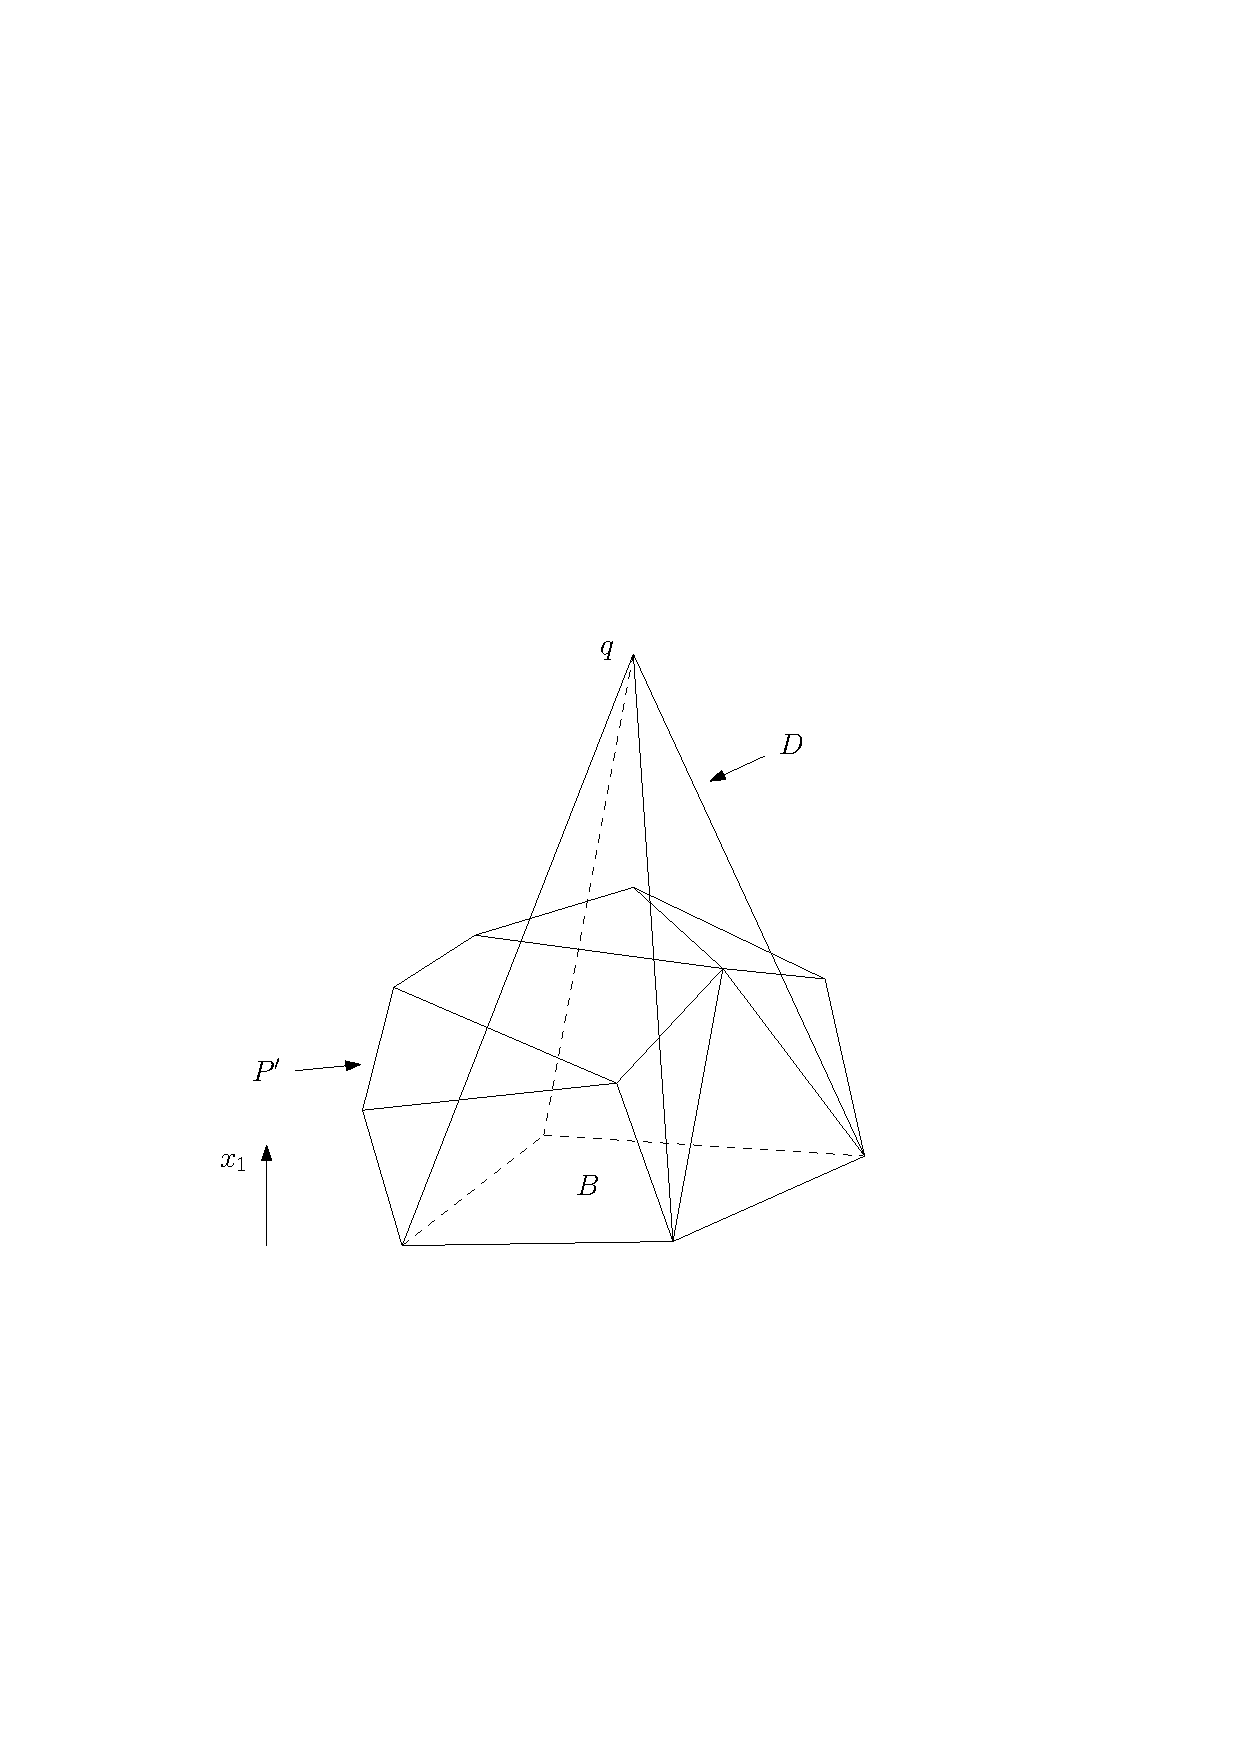
\includegraphics[width=0.35\textwidth]{pics/polpyr.pdf}
  }
  \hspace{10mm}
  \subfigure[]{\label{fig:rot}
    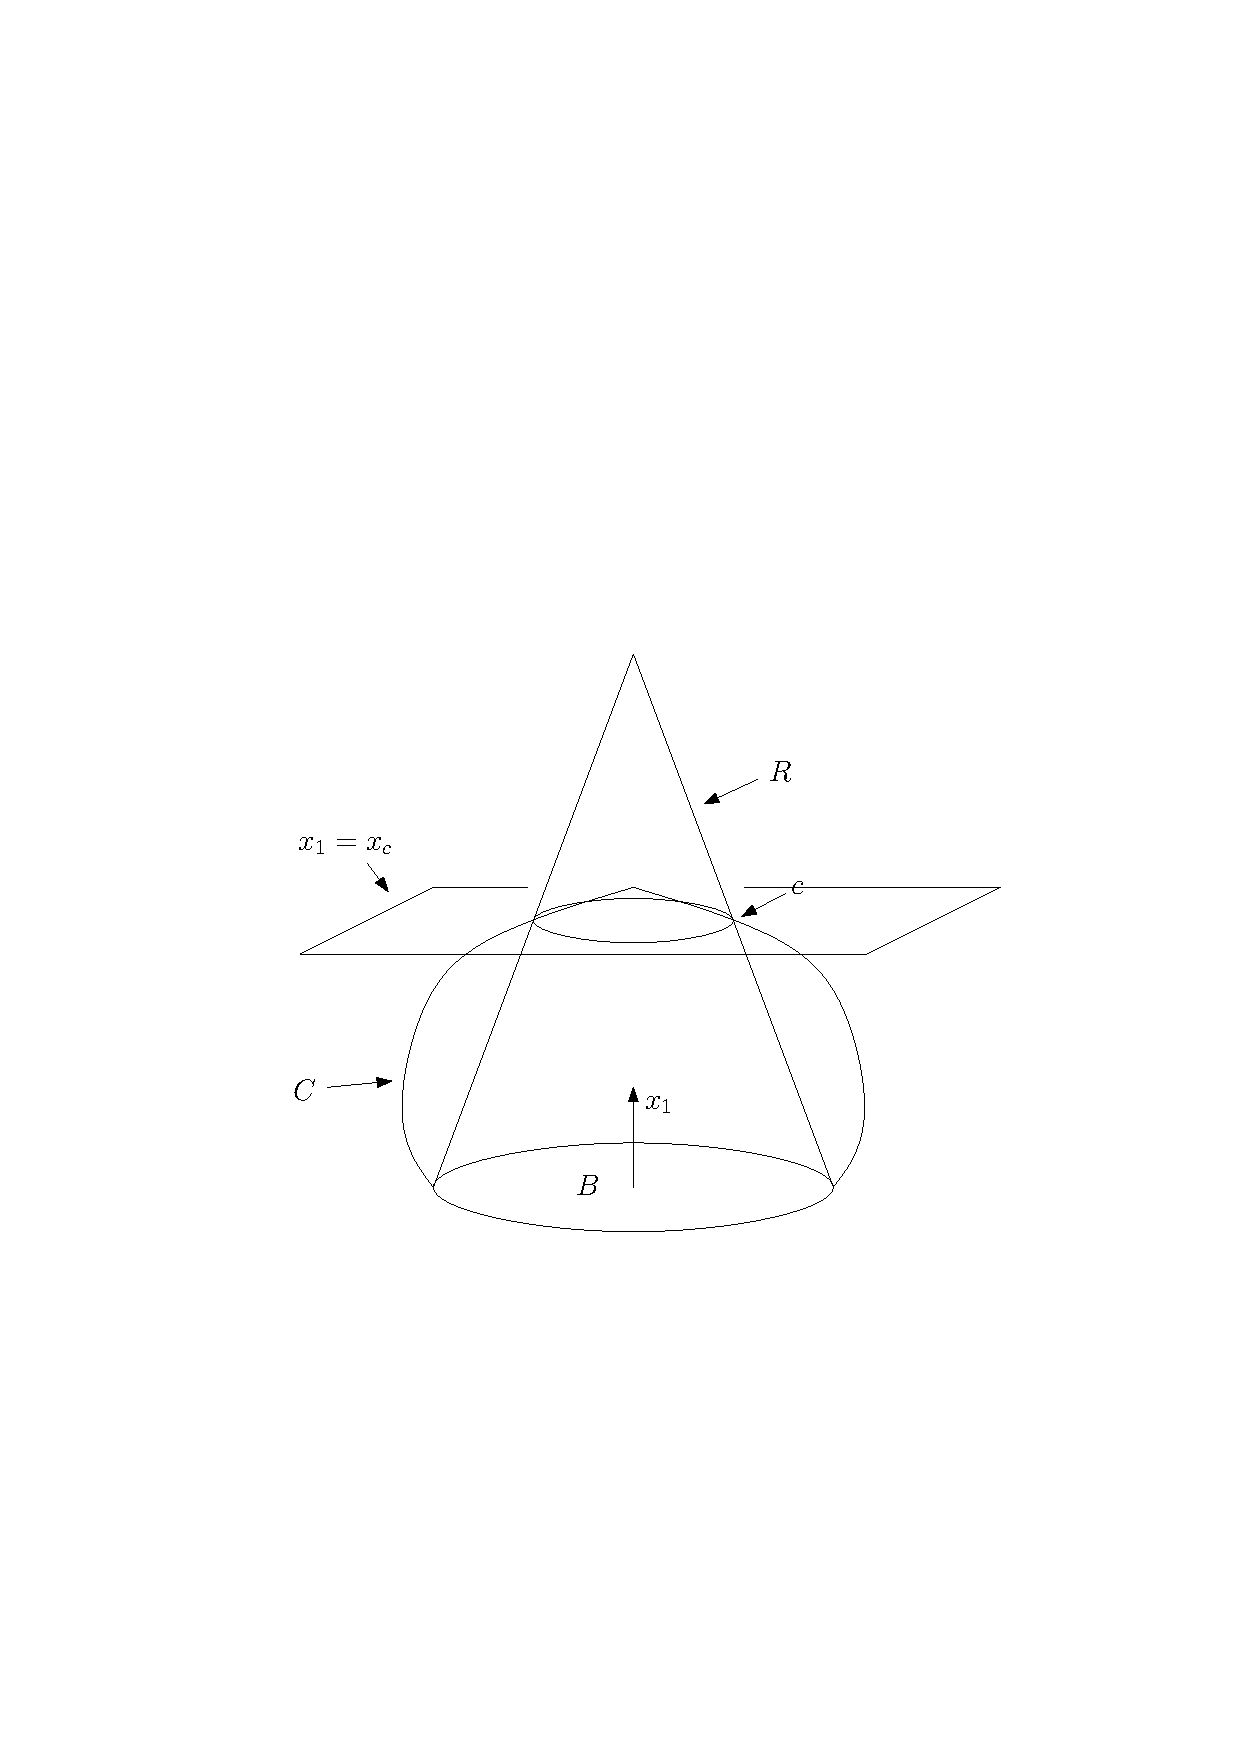
\includegraphics[width=0.39\textwidth]{pics/rotsym.pdf}
  }
  \caption{The Schwarz rotation-symmetral of $P'$ and $D$}
  \label{fig:rotsym}
\end{figure}

Let $x_{c}$ be the $x_{1}$-coordinate of $c$. Since
$C$ is convex. Then the surface of $C$ below
$x_{1} = x_{c}$ is outside the surface of $R$. By the definition of
Schwarz rotation-symmetral, the volume of $C$ that is outside of
$R$ is below $x_{c}$, and the volume of $R$ outside of $C$ is above
$x_{c}$. Therefore, the gravity center of $R$ is above that of $C$
because of central identity.

The gravity centers of $P'$ and $C$ have the same height because in the
Schwarz rotation-symmetral $C_{x}$ has the same $x_{1}$ value as $A_{x}$.
So do the gravity centers of $D$ and $S$. Let $g_{d}$ be gravity center of
$D$. Since $D$ is a pyramid, the convex hull of the $d$ points is contained
in $B$,  $g$ is below $g'$, and $g'$ is below $g_{d}$, so 
\[ \vol(T) \leq \vol(P')/(d+1) \leq \vol(P)/(d+1).\]
(To see this, consider that $\vol(T)\le\vol(g_d,p_1,\ldots,p_d)\le \vol(q',p_1,\ldots,p_d)/(d+1)$.)
\end{proof}

\begin{theorem}
  \label{thm:ndcenter}
  Let $S$ be a set of points in $\R^d$ whose convex hull, $A$, has unit volume. Then $\od(\cog(A),S)\le \binom{n}{d}/(d+1)$.
\end{theorem}

\begin{proof}
  According to Lemma~\ref{lem:simpvol},
  \[
    \begin{aligned}
     \od(\cog(A), S) 
      & = \sum_{y_{1},\ldots , y_{d} \in \binom{S}{d}} \vol(\cog(A), y_{1}, \ldots,
y_{d}) \\
      & \leq \binom{n}{d}/(d+1). 
    \end{aligned} \]
\end{proof}
% Does any other point has smaller upper bound?

\section{Oja Center and Gravity Center of $S$}
\label{sec:cnterofS}

In this section, we show that the center of gravity of $S$ provides a
constant-factor approximation to the point of minimum Oja depth.

\begin{theorem}
\label{thm:grav1d}
For any finite set $S\subset\mathbb{R}$, $\od(\cog(S),S) \le 2\od(x,S)$ for
any $x\in\mathbb{R}$.
\end{theorem}

\begin{proof}
Denote the elements of $S$ by $p_1,\ldots,p_n$ in any order.  Let the
multiset $S_i$ contain $p_1,\ldots,p_i$ as well as $n-i$ copies of
$x$. 
Let $c_i=\cog(S_i)$.
We will show, by induction on $i$, that $\od(c_i,S_i)\le
2\od(x,S_i)$ for all $i\in\{0,\ldots,n\}$.  This is sufficient,
since $S_n=S$.

For the base case $S_0$ consists of $n$ copies of $x$, so
$c_0=x$ and $\od(c_0,S_0)= 0 = 2\od(x,S_0)$.  Next,
we assume that $\od(c_i,S_i) \le 2\od(x,S_i)$ and prove that
$\od(c_{i+1},S_{i+1}) \le 2\od(x,S_{i+1})$.  Note that
\[
   \od(x,S_{i+1}) = \od(x,S_i) + |p_{i+1}-x| \enspace .
\]
Furthermore, 
\[
   c_{i+1} = c_i + (p_{i+1}-x)/n \enspace ,
\]
so
\begin{align*}
    \od(c_{i+1}, S_{i+1}) 
     & =  \od(c_i, S_{i}) \\ 
     &  \quad + \sum_{q\in S_i} (|c_{i+1} - q| - |c_i - q|) \\
     &    \quad + (|c_{i+1} - p_{i+1}| - |c_{i+1} - x|) \\
     & \le  \od(c_i, S_{i}) 
         \quad + n|p_{i+1}-x|/n  \\
    &    \quad + (|c_{i+1} - p_{i+1}| - |c_{i+1} - x|) \\
     & \le  \od(c_i, S_{i}) 
             + 2|p_{i+1}-x|  \\
     & \le  2\od(x, S_{i}) 
             + 2|p_{i+1}-x|  \\
     &  =  2\od(x, S_{i+1}) \enspace ,
\end{align*}
as required.
\end{proof}

We remark that the above proof uses little more than triangle
inequality. In particular, the same proof shows that the center of
gravity gives a 2-approximation for the Fermat-Weber center in any
dimension.\footnote{The Fermat-Weber center of a point set $S$ in $\R^d$
is the point $x$ that minimizes $\sum_{y\in S}\|x-y\|$.}  Unfortunately,
in higher dimensions, Oja depth does not enjoy this nice property.

\begin{theorem}
\label{thm:gravdd}
For any finite set $S\subseteq\mathbb{R}^d$,
$\od(\cog(S),S) \le (d+1)\od(x,S)$ for any $x\in\mathbb{R}^d$.
\end{theorem}

\begin{proof}
In this proof, we will make use of the fact that, for any $d$-simplex $T$ with vertex set $V_t$ and a point
$q\in\mathbb{R}^d$,
\begin{equation}
  \vol(T) \le \sum_{p_1,\ldots,p_d\in\binom{V_t}{d}} \vol(p_1,\ldots,p_d,q)\enspace , 
   \label{eq:cover}
\end{equation}
since $T$ is contained in the union of the simplices on the right hand side.

Define $S_i$ as in the proof of Theorem~\ref{thm:grav1d}. Let $S' = S_{i+1}\setminus \{p_{i+1}\}$ The induction
and base case are the same as in Theorem~\ref{thm:grav1d}. First, we have
\begin{eqnarray}
\od(x,S_{i+1}) 
   & = & \od(x,S_i) \nonumber \\
   && {} + \sum_{Q\in\binom{S_i}{d-1}} \vol(x,p_{i+1},Q), \label{eq:o}
\end{eqnarray}
where $Q$ is a set of $d-1$ points, and
\begin{align}
   & \!\!\! \od(c_{i+1},S_{i+1}) \nonumber \\
   & = \od(c_i,S_{i}) \nonumber \\
   &    \quad + \sum_{P \in \binom{S_i}{d}} 
           (\vol(c_{i+1}, P)- \vol(c_i,P))
              \label{eq:i} \\
   &   \quad + \sum_{Q\in \binom{S'}{d-1}}
           (\vol(c_{i+1},p_{i+1},Q)- \vol(c_{i+1},x,Q)),
            \label{eq:ii} 
\end{align}
where $P$ is a set of $d$ points.

First we show that $(\ref{eq:i}) \le (\ref{eq:o})$.
%By (\ref{eq:cover}), we can bound each term in (\ref{eq:i}) using the inequality
%   \[ \vol(c_{i+1},p,q)- \vol(c_i,p,q) 
%   \le 
%   \vol(p,c_i,c_{i+1}) + \vol(q,c_i,c_{i+1}) .\]
%(see Figure~\ref{fig:triangdiff}). 
%\begin{figure}[h]
%  \centering
%  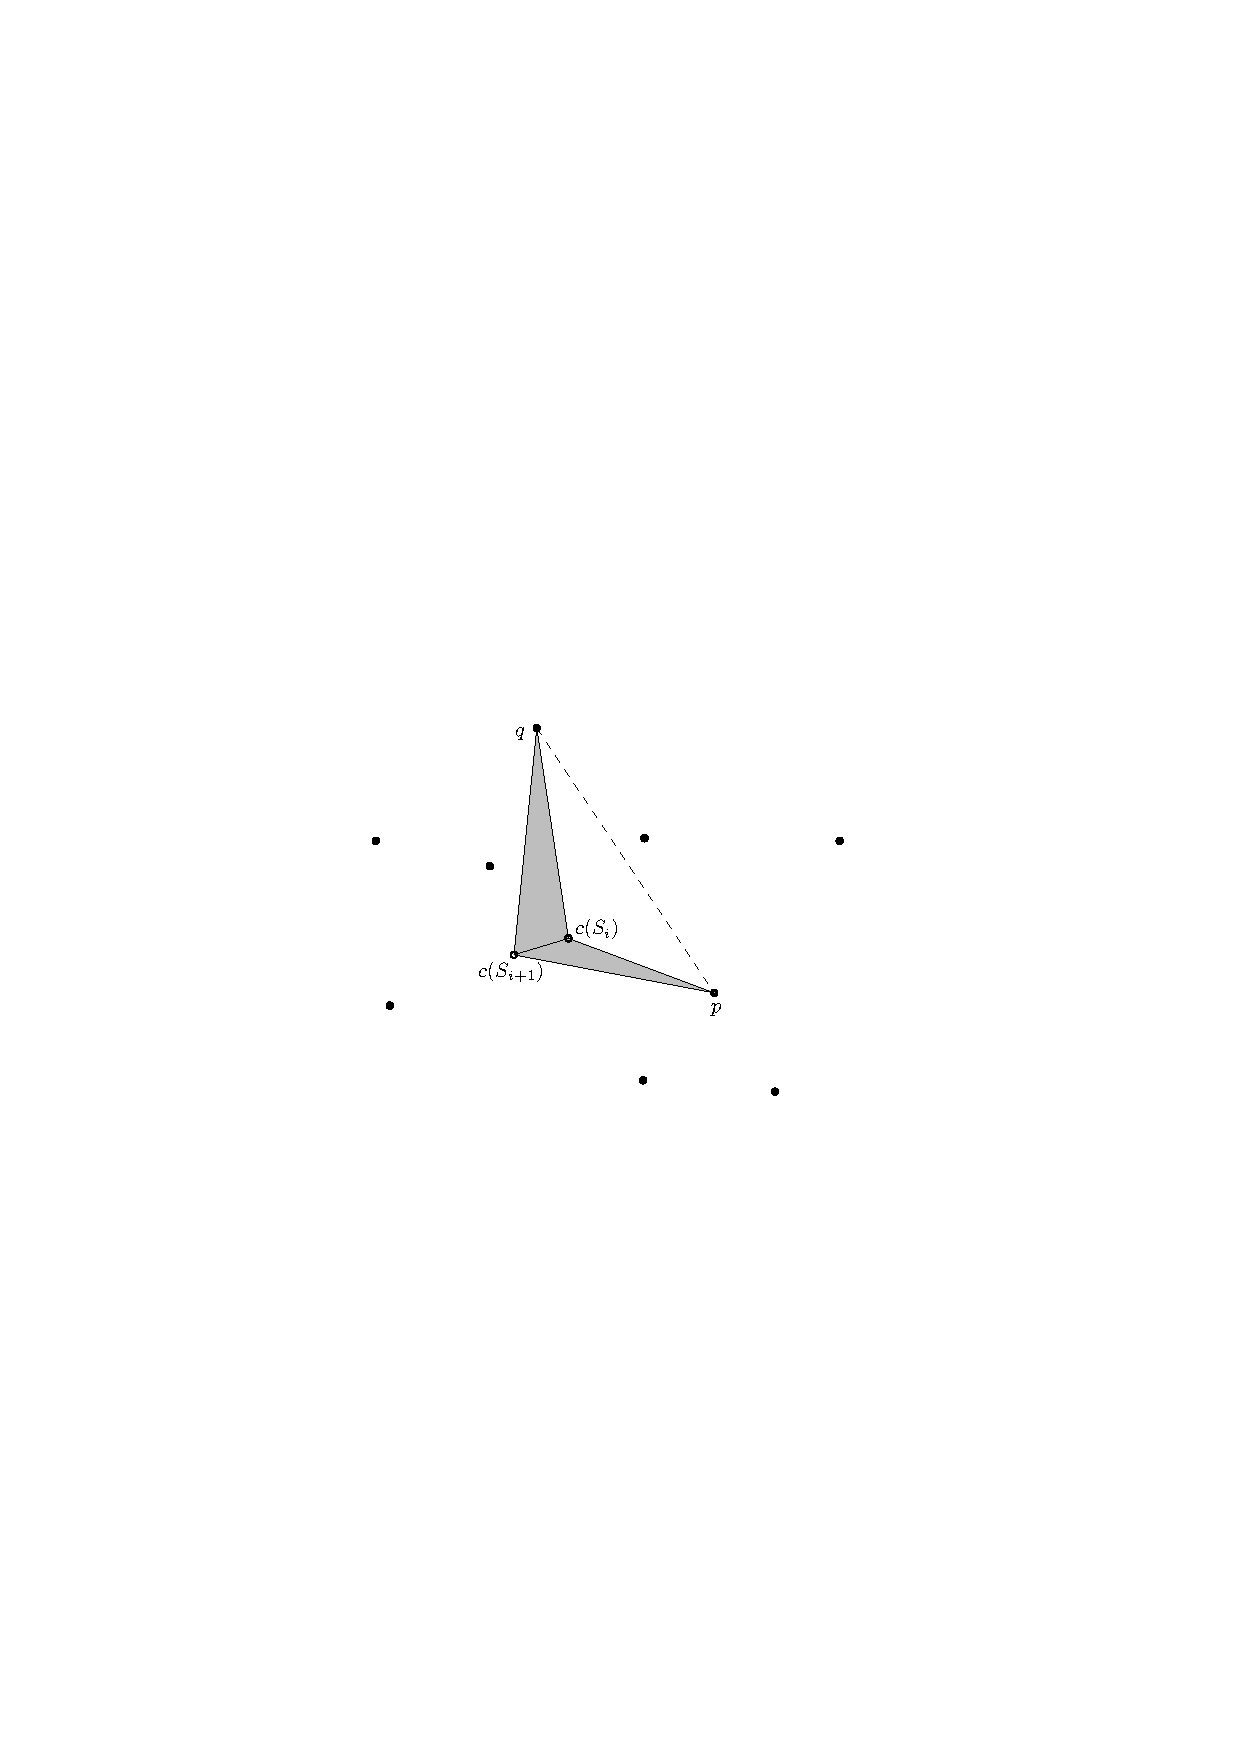
\includegraphics[width=.8\columnwidth]{pics/triangdiff.pdf}
%  \caption{The biggest difference}
%  \label{fig:triangdiff}
%\end{figure}
%On the right-hand side of the above inequality, there are two triangles each having a side at $c_i,c_{i+1}$.  Let $v_{i+1}=p_{i+1}-x$ and note that 
%$c_{i+1}-c_i = v_{i+1}/n$.  Therefore, 
%\[
% \vol(c_i,c_{i+1},p) = \frac{1}{2n}\cdot\|v_{i+1}\|\cdot\|(p_\drop-x_\drop)\|
%\]
%where $p_\drop$ denotes the orthogonal projection of $p$ onto some line
%orthogonal to $v_{i+1}$.  Therefore, we can bound \eqref{i} as
%\begin{align}
%   & \!\!\! \sum_{(p,q)\in S_i} (\vol(c_{i+1},p,q)- \vol(c_i,p,q)) 
%       \nonumber \\
%   &\le \sum_{\{p,q\}\in S_i}
%   (\vol(p,c_i,c_{i+1}) + \vol(q,c_i,c_{i+1}))  \\
%   & \le  (n-1)\sum_{p\in S_i} \vol(p,c_i,c_{i+1}) \\
%   & =  (1-1/n)\frac{1}{2}\|v_{i+1}\|\sum_{p\in
%S_i}(\|{c_{i+1}}_\drop-p_\drop\|) \\
%   & =  (1-1/n)\frac{1}{2}\|v_{i+1}\|\od({c_{i+1}}_\drop,
%\{p_\drop:p\in S_{i}\}) \\
%   & =  (1-1/n)\frac{1}{2}\|v_{i+1}\|\od({c_i}_\drop,
%\{p_\drop:p\in S_{i}\}) \\
%   & \le  (1-1/n)\|v_{i+1}\|\od(x_\drop, \{p_\drop:p\in S_{i}\})
%     \label{eq:drop} \\ 
%   & \le  \|v_{i+1}\|\od(x_\drop, \{p_\drop:p\in S_{i}\}) \\
%   & =  2\cdot \sum_{j=1}^i \vol(x,p_j,p_{i+1}) 
%\end{align}
%where inequality (\ref{eq:drop}) follows from Theorem~\ref{thm:grav1d}.

\[
  \begin{aligned}
  & \!\!\! \sum_{P \in \binom{S_i}{d}} (\vol(c_{i+1}, P)- \vol(c_i,P)) \\
  & \le \frac{1}{n} \sum_{P \in \binom{S_i}{d}} \left( \sum_{y \in S_{i+1}} \vol(y,P)  -  \sum_{y \in S_{i}} \vol(y,P)\right)\\
  & \le \frac{1}{n} \sum_{P \in \binom{S_i}{d}}( \vol(p_{i+1},P) - \vol(x,P)) \\
  & \le \frac{1}{n} \sum_{P \in \binom{S_i}{d}} \sum_{Q \in \binom{P}{d-1}} \vol(x,p_{i+1}, Q)  \\
  & \le \frac{n-(d-1)}{n} \sum_{Q \in \binom{S_i}{d-1}}  \vol(x,p_{i+1}, Q)  \enspace .
  \end{aligned}
\]
Next, we relate (\ref{eq:ii}) to (\ref{eq:o}) by showing that $(\ref{eq:ii}) \le d\times (\ref{eq:o})$. Applying (\ref{eq:cover}), we obtain
\[
  \begin{aligned}
     & \!\!\! \sum_{Q\in \binom{S'}{d-1}}
           (\vol(c_{i+1},p_{i+1},Q)- \vol(c_{i+1},x,Q)) \\
     &\le  \sum_{Q\in \binom{S'}{d-1}} 
           \left(\vol(x,p_{i+1},Q) + \sum_{R \in \binom{Q}{d-2}} \vol(x,p_{i+1},c_{i+1},R)\right) \\
     &\le  \sum_{Q \in \binom{S_i}{d-1}}  \vol(x,p_{i+1}, Q) \\
     & \quad + (n-1 - (d-2)) \sum_{R \in \binom{S_i}{d-2}} \vol(x,p_{i+1},c_{i+1},R) \enspace ,
  \end{aligned}
\]
where $R$ is a set of $d-2$ points. By linearity of determinant we have
\[
  \begin{aligned}
  \vol(x,p_{i+1},c_{i+1},R) & = \frac{1}{n} \sum_{y \in S_{i+1}} \vol(x,p_{i+1},y,R) \\
  & = \frac{1}{n} \sum_{y \in S_{i}} \vol(x,p_{i+1},y,R)
  \end{aligned}
\]
and thus
\[
\sum_{R \in \binom{S_i}{d-2}} \vol(x,p_{i+1},c_{i+1},R) = \frac{d-1}{n}\sum_{Q \in \binom{S_i}{d-1}}  \vol(x,p_{i+1}, Q).
\]
Thus we can get $(\ref{eq:ii}) \le d\times (\ref{eq:o})$.


Finally, we resubstitute to obtain
\[
  \begin{aligned}
     & \!\!\! \od(c_{i+1},S_{i+1}) \\
     &\le \od(c_{i},S_{i}) + (d+1) \sum_{Q\in\binom{S_i}{d-1}} \vol(x,p_{i+1},Q)\\
     &\le (d+1) \od(x,S_{i}) + (d+1) \sum_{Q\in\binom{S_i}{d-1}} \vol(x,p_{i+1},Q) \\
     & = (d+1) \od(x,S_{i+1})  \enspace .
  \end{aligned}
\]
as required.
\end{proof}

We remark that Theorem~\ref{thm:grav1d} and~\ref{thm:gravdd} are essentially the best possible. To see this, take the multiset $S$ that contains $n-d$ copies of the origin $o$, and each of the remaining $d$ points has one different coordinate $1$ and all other coordinates $0$. In this case $\od(o, S)= 1/d!$ and $\od(\cog(S), S)= (d + 1 - O(d^2/n))\times 1/d!$.

\section{Conclusion}
\label{sec:concl}

We have given several results on Oja depth and centers of gravity.
There are several directions for future work.

Theorem~\ref{thm:ndcenter} has no matching lower bound.  The best lower-bound
we know is that placing $n/(d+1)$ points at each of the vertices of a
point center whose Oja center $x$ has Oja depth $n^d / (d+1)^{d-1}$.
For $d=2$, for example, Theorem~\ref{thm:ndcenter} implies $\od(x, S)\le n^2/6
- O(n)$ where as the best lower bound (above) has $\od(x, S)\ge n^2/9$.
This construction leads us to our first conjecture:
\begin{conj}
For any point set $S\subset\R^d$ whose convex hull has unit volume, there exists $x\in\R^d$, such that $\od(x,S)\le n^d / (d+1)^{d-1}$
\end{conj}


\small 
\bibliographystyle{abbrv}
\bibliography{ojacenter}

\end{document}
